\section{Scelte Progettuali PoC}
\subsection{Introduzione}



\subsection{Introduzione}
In questa sezione verranno descritte le scelte progettuali del PoC, i compromessi legati alle tecnologie usate e quello che non traspare dal codice stesso.



\subsection{Tecnologie Usate}
\begin{itemize}
\item{Java 1.8:} era un requisito definito a priori visto l'uso massiccio che ne fa XTN con Smash.
\item{Spring Boot:} era un prerequisito che mi ha facilitato molto per creare e testare i vari progetti stand-alone .
\item{Spring Data Neo4j:} progetto derivato da Spring Data astrarre i driver Java per Neo4j, fare il mapping delle classi Java, annotate come entity, nel contesto di Neo4j e facilitare le ricerche nel grafo.
\item{Maven:} software usato per la gestione dei progetti Java.
\item{Tinkerpop/BluePrints:} visto che Spring Data OrientDB \'e un progetto acerbo e senza documentazione \'e stato preferito usare Tinkerpop per interfacciarsi con OrientDB.
\item{JUnit e Mockito:} usato per create unit test.
\item{Macchina virtuale:} \'e stata resa disponibile una macchina virtuale con xeon e5-1650 3.50ghz, 4gb di ram e 34gb di spazio disponibile per il mio account.
\item{Docker:} tutti i test sono stati eseguiti nella macchina virtuale sotto ambiente Docker.
\end{itemize}
\newpage
\subsection{Diagramma dei Package}
Il PoC \'e stato diviso in vari progetti Maven sotto l'unico progetto aggregato chiamato \textit{xtn\textunderscore research\textunderscore graphdbs}, questo per avere un progetto padre per gestire tutte le versioni delle dipendenza in un unico Pom e avere la comodit\'a di eseguire la build di tutti i progetti in un unico comando lasciando Maven a risolvere le dipendenze.

\begin{figure}[ht]
	\centering
	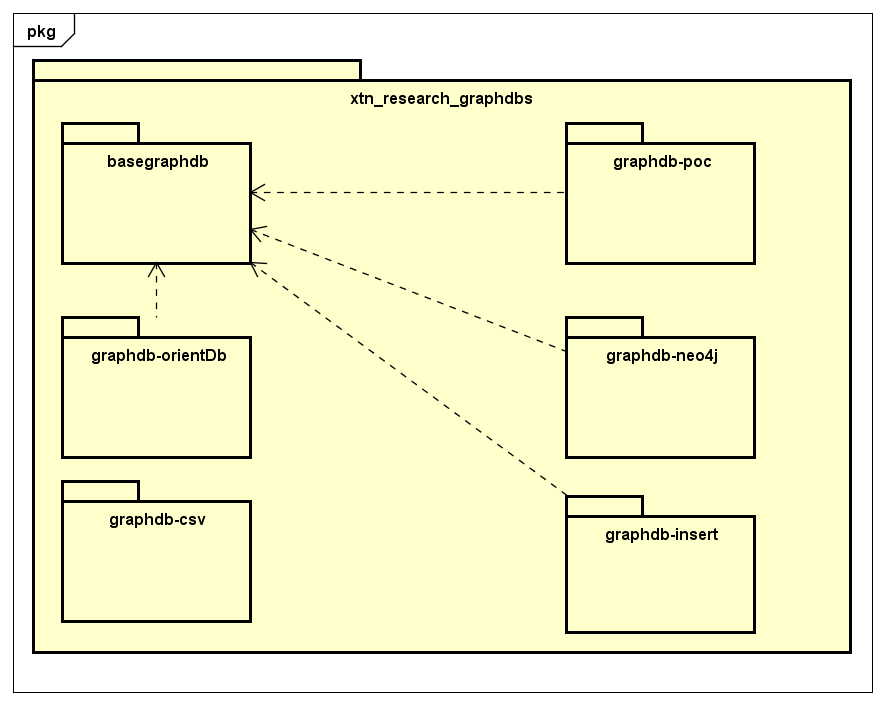
\includegraphics[scale=0.70]{diagram/img/packages.png}
	\caption{Packages}
\end{figure}

\subsubsection{basegraphdb}
Basegraphdb \'e il progetto cui contiene le varie interfacce comuni tra cui la classe \textit{ReputationController} e la classe \textit{Transaction}.
\textit{ReputationController} \'e l'interfaccia comune per gestire la reputazione delle varie entit\'a presente nei vari Database, ogni implementazione, quindi sia graphdb-neo4j, sia graphdb-orientDb che qualsiasi altra futura implementazione, ha all'interno una classe che la implementer\'a. \textit{Transaction} invece \'e una classe concreta che rappresenta una transazione indipendentemente da che implementazione di un qualsiasi database si voglia usare, l' oggetto \textit{Transaction} \'e costruito tramite l'oggetto \textit{TransactionBuilder} visto i molti parametri necessari.

\subsubsection{graphdb-orientdb}
Graphdb-orientDb \'e il progetto per la gestione della reputazione tramite OrientDB, esso ha all'interno una classe chiamata \textit{ReputationControllerOrientDb} che implementa la classe base \textit{ReputationController} contenuta nel package \textit{basegraphdb} descritta precedentemente. Questa implementazione usa Tinkerpop/BluePrints come astrazione per la gestione delle chiamate REST per l'aggiunta, modifica e interrogazione del database.

\subsubsection{graphdb-neo4j}
Graphdb-neo4j \'e il progetto per la gestione della reputazione tramite Neo4j, esso ha all'interno una classe chiamata \textit{ReputationControllerNeo4j} che implementa la classe base \textit{ReputationController} contenuta nel package \textit{basegraphdb} descritta precedentemente. Questa implementazione usa Spring Data Neo4j come astrazione per per la gestione delle chiamate REST per l'aggiunta, modifica e interrogazione del database tramite semplici annotazioni. All'interno del packag, inoltre, sono presenti tutte le classi necessarie a Spring Data per la generazione di codice sorgente come le varie classi annotate come textit{@NodeEntity} che rappresentano i nodi del grafo, oppure le varie Repository per la gestione dell'input/output del database.
Le classi annotate come \textit{@NodeEntity,@RelationshipEntity} non \'e stato possibile segnarle con visibilit\'a package, anche se sarebbe stato corretto, a causa di Spring Data Neo4j.

\subsubsection{graphdb-poc}
Graphdb-poc il progetto che si occupa solamente di istanziare le varie implementazioni di \textit{ReputationController} contenuto nel package textit{basegraphdb} ed eseguire i vari metodi tracciando, e stampando a video, il nome del metodo chiamato, il risultato ottenuto, il tipo di database che l'ha calcolato ed il tempo impiegato in millisecondi.
Questo progetto ha solamente una dipendenza verso l'interfaccia comune, l'onere di iniettare le varie dipendenze con le implementazioni viene lasciato totalmente a Spring, in questo modo si ha un disaccoppiamento tra il PoC e le varie implementazioni e, sopratutto, se in futuro ci fosse il bisogno di aggiungere un altra implementazione di \textit{ReputationController} non ci sarebbe bisogno di modificare il codice di questo progetto.

\subsubsection{graphdb-csv}
Graphdb-csv \'e il progetto per creare i diversi documenti csv contenenti le entit\'a per popolare i diversi tipi da database, questo progetto crea 4 diversi documenti csv nella root del progetto:
\begin{itemize}
\item{\textbf{account.csv:}} contenente una sola colonna con l'id del account, ad esempio l'IBAN di un conto bancario.
\item{\textbf{entity.csv:}} contenente una sola colonna con l'id di una entit\'a che ha stipulato un contratto con una banca, un entity pu\'o avere da 0 a n account associati a lui.
\item{\textbf{entity\textunderscore account.csv:}} contenente 2 colonne, un id di un entity e uno di un account, che rappresentano l'appartenenza di un account ad un entity.
\item{\textbf{transaction.csv:}} contenente tutte le informazioni di una transazione comprese il payee ed il payer.
\end{itemize}
Questo progetto crea i dati nel migliore di casi, cio\'e che ogni account ha sempre il suo entity associato.


\subsubsection{graphdb-insert}
Graphdb-insert \'e il progetto che dato il numero di account, entity e transazioni li crea nel modo del tutto casuale e li aggiunge nel database scelto. Questo progetto utilizza l'interfaccia comune \textit{ReputationController} per aggiungerli in modo indipendente all'implementazione usata.//
\textbf{Usare questa classe solo per aggiungere un basso numero di nodi visto che viene aggiunto un record in circa 500ms, in caso contrario \'e pi\'u efficiente generarsi il csv con il progetto descritto precedentemente ed utilizzare l'importatore csv nativo del database}

\subsection{Ambiente di test}
I test sono stati scritti sopo aver sviluppato il codice e sono stati testati solo i componenti non banali che utilizzavano solo librerie importare, per non rischiare di testare codice già testato da altri. \'E stato utilizzato Mockito per creare un mock dei repositori per facilitare i test che utilizzavano queste classi, invece per testare i repository sono state vere istanze di orientDb e Neo4j.
\subsubsection{Requisiti per eseguire i test}
\begin{itemize}
\item{Neo4j}: un istanza di neo4j con:
\begin{itemize}
\item{username:} neo4j
\item{password:} password
\item{Porta http:} http://127.0.0.1:7473
\end{itemize}
\item{OrientDB:} un istanza di orientDB
\begin{itemize}
\item{username:} admin
\item{password:} admin
\item{database:} un database chiamato \textit{xtn\textunderscore graph} con il seguente schema:
\begin{itemize}
\item{BaseAccount:} Una classe \textit{BaseAccount} astratta che estende da \textit{V}
\item{EntityId} Una classe \textit{EntityId} concreta che estende da \textit{V} e \textit{BaseAccount} che ha un campo dati di tipo String chiamato \textit{entityId}, ed esso \'e un indice di tipo unique.
\textit{AccountId} che ha un campo dati di tipo String chiamato \textit{accountId}, ed esso \'e un indice di tipo unique.
\item{OWN:} una classe chiamata \textit{OWN} che estende \textit{E}
\item{TRANSACTION}: una classe chiamata \textit{TRANSACTION} che estende \textit{E}
\end{itemize}
\item{Porta http:} http://127.0.0.1:7473
\end{itemize}
\end{itemize}



